\documentclass[11pt, oneside, a4paper]{article}
%\usepackage[cp1251]{inputenc} % кодировка
\usepackage[utf8]{inputenc} % кодировка
\usepackage[english, russian]{babel} % Русские и английские переносы
\usepackage{graphicx}          % для включения графических изображений
\usepackage{cite}              % для корректного оформления литературы
\usepackage{enumitem}
\usepackage{pavt-ru}  

\usepackage{amsmath, amssymb}

\begin{document}

% \title - название статьи
% \authors - список авторов

\title{Оптимизация значений гиперпараметров нейросетевой модели классификации и сегментации сигналов ЭКГ \footnote{Работа выполнена при поддержке программы стратегического академического лидерства <<Приоритет 2030>>.}}

\authors{ Д.А.~Ануфриев, Е.Н.~Варсеева, А.С.~Зайцев, Е.Г.~Голдинова, К.С.~Егоров, М.А.~Усова, Д.А.~Карчков, И.Г.~Лебедев, К.А.~Баркалов}
\organizations{ Нижегородский государственный университет им. Н.И. Лобачевского }

% Аннотация заключается в окружение abstract
\begin{abstract}
В статье рассматривается задача оптимизации гиперпараметров нейросетевой модели классификации и сегментации сигналов электрокардиограммы (ЭКГ) с использованием программной системы Globalizer. Объектом исследования являются архитектуры нейросетей MobileNetV3 Small и U-Net 1D, направленных на решение задачи классификации и сегментации соответственно, адаптированные для обработки 10-секундных фрагментов ЭКГ, записанных с частотой дискретизации 500 Гц. 
Задача классификации заключается в определении ведущего ритма сердечной деятельности: синусовый ритм, синусовые вариации, другие типы ритма. Задача сегментации направлена на локализацию в сигнале базовых элементов кардиоцикла, соответствующих сокращению предсердий сердца, желудочков и восстановлению миокарда. 
%Варьируемыми гиперпараметрами выступают число классифицирующих нейронов в выходном слое (80–200) и вероятность Dropout (0.0–1.0) для классифицирующей нейронной сети, и количество уровней архитектуры (2-5) и вероятность Dropout (0.0–1.0) для сегментирующей. 
Для решения задачи настройки гиперпараметров применен информационно-статистический алгоритм глобального поиска, реализованный в системе Globalizer и принадлежащий классу методов липшицевой глобальной оптимизации. 
%Алгоритм является детерминированным, что обеспечивает воспроизводимость результатов и гарантированную сходимость к глобальному оптимуму.
Представлены результаты сравнения эффективности Globalizer с известными фреймворками Optuna и HyperOpt, демонстрирующие сопоставимое качество оптимизации при существенном сокращении времени настройки. Полученные результаты подтверждают перспективность применения детерминированных методов липшицевой оптимизации для точной настройки гиперпараметров глубоких нейронных сетей в медицинских диагностических задачах.
\end{abstract}

\keywords{глобальная оптимизация, многоэкстремальные функции, параллельные вычисления, нейронные сети, искусственный интеллект}

% \section{название} - заголовок раздела первого уровня
% \subsection{название} - заголовок раздела второго уровня
% \subsubsection{название} - заголовок раздела третьего уровня
% Не используйте уровень вложенности заголовков больше трех!
% Каждый абзац текста в статье начинается командой \par или пустой
% строкой.


\section{Введение}
\label{sec-intro}

Электрокардиография (ЭКГ) является одним из наиболее распространенных и информативных методов диагностики сердечно-сосудистых заболеваний. Ежегодно в мире регистрируются миллионы электрокардиограмм, и автоматический анализ этих данных представляет собой актуальную задачу медицинской информатики. В последние годы для классификации ЭКГ-сигналов активно применяются методы глубокого обучения, в частности сверточные нейронные сети, которые демонстрируют высокую точность при решении задач распознавания ритмов и выявления аномалий \cite{Ansari2023,  Seenivasan2025, Xiao2023, Huang2023}. Однако эффективность таких моделей существенно зависит от правильного выбора гиперпараметров --- значений, определяющих архитектуру сети и процесс ее обучения.

Задача оптимизации гиперпараметров моделей ИИ заключается в поиске такой комбинации гиперпараметров, которая обеспечивает наилучшее значение целевой метрики качества модели. С математической точки зрения эта задача относится к классу задач глобальной оптимизации с ограничениями, причем целевая функция, как правило, является многоэкстремальной, не имеет аналитического описания (представляет собой <<черный ящик>>), а ее однократное вычисление требует значительных вычислительных ресурсов, связанных с обучением нейронной сети. Указанные особенности делают задачу оптимизации гиперпараметров чрезвычайно сложной и требуют развитие специализированных методов оптимизации.

Среди наиболее известных фреймворков для автоматической настройки гиперпараметров можно выделить Optuna \cite{optuna} и HyperOpt \cite{hyperopt}, которые реализуют байесовские методы оптимизации, случайный поиск, а также эволюционные и генетические алгоритмы \cite{Yang2013,Gendreau2010,Eiben2015}. Эти подходы являются стохастическими по своей природе, что приводит к вариабельности результатов при многократных запусках и не гарантирует нахождения глобального оптимума за ограниченное число итераций. Альтернативой стохастическим методам выступают детерминированные алгоритмы глобальной оптимизации \cite{Kvasov2018,Sergeyev2006,Zilinskas2008}, одним из которых является информационно-статистический алгоритм глобального поиска, разработанный в Нижегородском государственном университете им. Н.И. Лобачевского \cite{Strongin2000, Strongin2018}. Данный алгоритм основан на предположении липшицевости целевой функции и использует редукцию размерности с помощью кривых Пеано для сведения многомерной задачи к одномерной. Важным преимуществом этого подхода является его детерминированность, обеспечивающая воспроизводимость результатов и гарантированную сходимость к глобальному минимуму при выполнении определенных условий \cite{Strongin2000}.

Программная реализация описанных методов выполнена в виде программной системы Globalizer (доступна в открытом репозитории \url{https://github.com/OptimLLab/Globalizer}), которая предназначена для решения задач выбора оптимальных параметров сложных систем, включая модели искусственного интеллекта и машинного обучения. Система поддерживает работу с частично целочисленными переменными, невыпуклыми ограничениями, а также предоставляет возможности для параллельных вычислений с использованием технологий OpenMP, MPI и CUDA.

Настоящая статья посвящена применению программной системы Globalizer для оптимизации гиперпараметров модели классификации и сегментации сигналов ЭКГ. В качестве базовых архитектуры классифицирующей сети выбрана адаптированная версия MobileNetV3 Small --- легковесная сверточной нейронной сети. Модель предназначена для классификации 10-секундных фрагментов ЭКГ, зарегистрированных в двух отведениях с частотой дискретизации 500 Гц. Задача классификации заключается в определении ведущего ритма сердечной деятельности: синусовый ритм, синусовые вариации или другие типы ритма. Варьируемыми гиперпараметрами являются число классифицирующих нейронов в выходном слое (в диапазоне от 80 до 200) и вероятность отключения нейронов (Dropout, в диапазоне от 0.0 до 1.0). Для решения задачи сегментации сигнала ЭКГ с целью локализации моментов активации предсердий, желудочков и восстановления миокарда используется архитектура U-Net, адаптированная для анализа одномерных сигналов. В угоду потоковой обработки ЭКГ средствами данной нейросетевой модели решено сформировать обучающую и тестовую выборку из участков 12-ти канальных сигналов, длительностью 1 секунда, или 500 отсчетов, что гарантирует попадание хотя бы одного кардиоцикла полностью или частично. Варьируемыми гиперпараметрами являются количество уровней архитектуры (значение глубины изменяется от 2 до 5), что позволяет параметрически изменять архитектуру сети и, как следствие, количество обучаемых параметров, а также вероятность отключения нейронов, используемая для регуляризации и предотвращения переобучения.


В качестве исходных данных для обучения и тестирования используется расширенный датасет LUDB \cite{Kalyakulina2020}, который содержит записи ЭКГ с метками как для задачи сегментации, так и для задачи классификации. LUDB является репрезентативной базой данных, широко применяемой в исследованиях по автоматическому анализу электрокардиограмм.

Статья имеет следующую структуру. В разделе 2 приводится постановка задачи оптимизации гиперпараметров и формальное описание используемой модели классификации ЭКГ. Раздел 3 содержит описание параллельного алгоритма глобального поиска. В разделе 4 описывается методика проведения вычислительных экспериментов, включая характеристики использованного вычислительного оборудования, параметры запуска алгоритмов и критерии сравнения. Раздел 5 посвящен анализу полученных результатов. В заключении сформулированы основные выводы и намечены направления дальнейших исследований.

\section{Постановка задачи}
\label{sec-problem}

Разработка диагностических алгоритмов, позволяющих определять наличие конкретной нозологии в сигнале ЭКГ, может базироваться на одной из фундаментальных задачах машинного обучения: задача классификации или задачи сегментации.

\subsection{Задача классификации}
Задача классификации в контексте машинного обучения сводится к отнесению исследуемого объекта к одному из заранее известных классов или категорий. 
При разработке нейросетевой модели, предпочтение отдано архитектуре, решающую задачу мультиклассовой классификации, при которой каждый сигнал относится только к одному классу.
В основу задачи классификации ЭКГ сигналов заложено разделение всех сигналов по типу ритма:
\begin{itemize}
  \item Синусовый ритм: нормальный ритм и его физиологические вариации;
  \item Cинусовые вариации: синусовая аритмия, брадикардия, тахикардия и др.;
  \item Другой ритм: предсердный, атриовентрикулярный, идиовентрикулярный и др.
\end{itemize}

Таким образом, поставлена задача разработки и обучения нейросетевой модели, адаптированной под классификацию сигналов ЭКГ, при условии варьирования параметров модели, таких как:
\begin{itemize}
  \item Число классифицирующих нейронов: в диапазоне от 80 до 200;
  \item Вероятность отключения нейронов (Dropout): в диапазоне от 0.0 до 1.0.
\end{itemize}
Важно отметить, что полученная модель в дальнейшем должна быть интегрирована в SoC микроконтроллер, для локального выделения нозологий на устройстве сбора данных без привлечения персональных компьютеров и серверных мощностей.

\subsubsection{Описание данных}
Обучающая и тестовая выборка сформирована из сигналов открытого датасета Lobachevsky University Electrocardiography Database, содержащего 200 аннотированных сигналов ЭКГ \cite{Kalyakulina2020}. Регистрация сигнала проводилась в 12-ти стандартных отведениях с частотой дискретизации 500 Гц в течении 10 секунд. Пример сигнала из датасета представлен на рис.~\ref{fig:ecgexample}.

\begin{figure}[h]
\centering
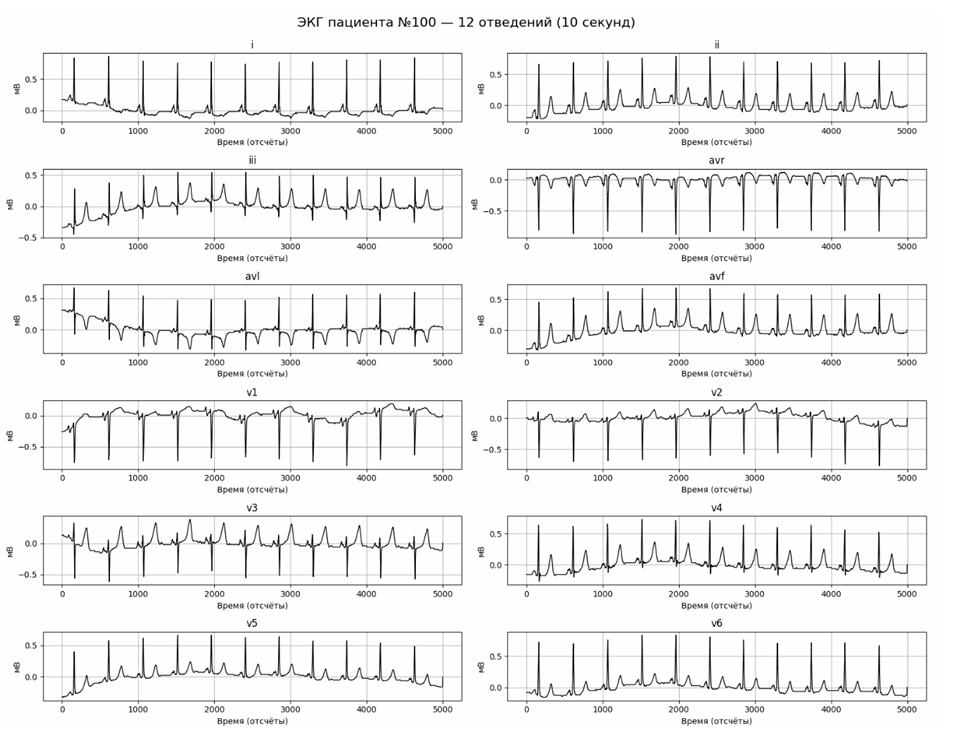
\includegraphics[width=1\textwidth]{ECGExample.png}
\caption{Образец ЭКГ сигнала в базе данных Lobachevsky University Electrocardiography Database, с отдельным отображением профиля каждого отведения}
\label{fig:ecgexample}
\end{figure}


Согласно описанию, записи в датасете, в зависимости от ритма, распределены следующим образом:
\begin{itemize}
  \item Синусовый ритм: 143;
  \item Синусовая тахикардия: 4;
  \item Синусовая брадикардия: 25;
  \item Синусовая аритмия: 8;
  \item Нерегулярный синусовый ритм: 2;
  \item Аномальный ритм 19.
\end{itemize}

С целью уменьшения размера итоговой модели при формировании обучающей и тестовой выборки выбраны первое (I) и второе (II) отведение. Кроме того, с медицинской точки зрения выбранные типы ритма хорошо представлены на графиках данных отведений, поэтому исключение остальных отведений из выборки не должно отрицательно сказаться на качестве классификации. 

Таким образом, при разделении датасета на 80\% обучающей выборки и 20\% тестовой выборки мы имеем соответственно 160 и 40 примеров размером (2 х 5000).

\subsubsection{Архитектура нейронной сети}
В силу ограниченного объема оперативной памяти на устройстве инференса базовой архитектурой выбрана MobileNetV3 Small, адаптированная под входные данные в формате (batch, 2, 5000). Графически архитектура представлена на рис.~\ref{fig:custommobilenet}.

\begin{figure}[h]
\centering
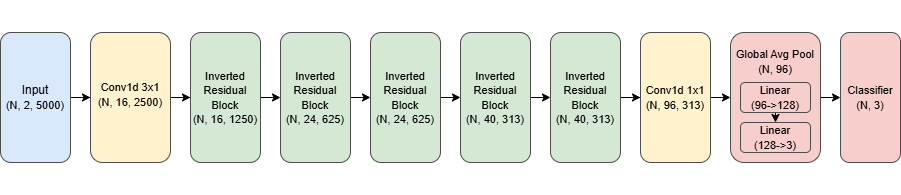
\includegraphics[width=1\textwidth]{CustomMobileNet.drawio.png}
\caption{ Графическое представление архитектуры MobileNetV3 Small, адаптированной под классификацию сигнала ЭКГ по двум отведениям}
\label{fig:custommobilenet}
\end{figure}

Применение блоков с инвертированными остаточными связями (inverted residual) позволяет сети не разрастаться, сохраняя малое число параметров и компактный размер, что важно при работе на SoC устройствах. Слой усреднения по глобальному окну (Global Average Pooling) позволяет агрегировать временную информацию, делая выход сети инвариантным к локальным сдвигам, что позволяет концентрироваться на наличии паттерна конкретной нозологии в сигнале ЭКГ, а не на его локализации в сигнале.

Для обучения модели использовался фреймворк машинного обучения PyTorch. Данный инструмент поддерживает автоматическое дифференцирование, адаптивен для разработки модифицированных архитектур с возможностью контроля их параметров, но главное --- позволяет использовать мощности GPU карт при обучении. Описанные особенности упрощают возможность оптимизации гиперпараметров нейросетевой модели при ее обучении.

Оптимизатор Adam (адаптивный метод оптимизации на основе градиентного спуска) хорошо справляется с разреженными градиентами, встречающихся в свертках, а также обеспечивает быструю сходимость на первых эпохах обучения.

В качестве функции потерь выбрана кросс-энтропийная функция (CrossEntropyLoss), представляющая собой комбинацию логарифмического SoftMax (LogSoftmax) и отрицательного логарифмического правдоподобия (Negative Log Likelihood), штрафующая модель, если вероятность правильного класса низкая. Данная функция потерь считается лучшей практикой при многоклассовой классификации в силу отсутствия проблемы взрыва или затухания градиента при сохранении интерпретируемости.

Параметр скорости обучения (Learning Rate) установлен в 1e-3, при этом оптимизатор Adam адаптивно меняет скорость для каждого веса. В качестве метрики качества классификации использовалась F1-мера, в силу сильного дисбаланса классов.

\subsection{Задача сегментации}

Сегментацией в кардиологии называют выделение в ЭКГ сигнале всех элементов кардиоциклов, соответствующих сокращению предсердий, желудочков и восстановлению миокарда. Точная локализация элементов кардиоциклов позволит однозначно определить нозологию, описанную в медицинской литературе, что позволит разработчику написать аналитический алгоритм.

Сегментация сигнала ЭКГ является не тривиальной задачей из-за существования низкоамплитудных зубцов, описывающих работу сердечной мышцы, в следствии чего интерпретация сигнала затрудняется и приводит к ошибочной диагностике.

Наиболее эффективный способ сегментации ЭКГ сигналов состоит в применении  нейронных сетей, изначально специализированных на сегментации изображений. Однако обучение таких моделей осложнено наличием гиперпараметров, для которых требуется точная настройка.

Таким образом, необходимо разработать нейросетевую модель, для решения задачи сегментации (выделения компонентов кардиоциклов) сигнала ЭКГ, и выбрать оптимальные значения ее гиперпараметров.

\subsubsection{Описание данных}
Исходные данные представляют собой набор json файлов, где каждый сигнал описывается двумя файлами: 
\begin{itemize}
  \item Файл с мета информацией о записи;
  \item Файл с сигналом и временными метками комплексов.
\end{itemize}
При формировании датасета использовалось 680 сигналов ЭКГ, локализацию сегментов в которых осуществляли врачи функционалисты, разрабатывающих первую версию базы данных Lobachevsky University Electrocardiography Database \cite{Kalyakulina2020}. Для обучения моделей сегментации каждая запись была преобразована в набор окон фиксированной длины с покомпонентной разметкой.


Основные шаг в подготовке датасета:
\begin{enumerate}
  \item Чтение сигнала. Для каждой записи считывается сигнал размера [число сэмплов окна, число входных каналов];
  \item Построение меток по каждому каналу. Для каждого канала отдельно считывается соответствующий файл аннотаций;
  \item Полученные файлы аннотаций переводятся в покомпонентный вектор меток числа сэмплов окна. Для классов поддерживается общий словарь: фон = 0, остальные классы нумеруются с 1;
  \item Для удаления неразмеченных участков применяется обрезка отсчетов с начала и конца. Если после обрезки длина записи меньше размера окна, запись исключается из рассмотрения.
  \item Нарезка на окна с перекрытием. Сигнал разбивается на окна длиной $W_s$ с заданным перекрытием. % overlap (stride = window\_size - overlap).
\end{enumerate}

Длина исходной записи составляет порядка 5000 отсчетов. Перед нарезкой выполняется обрезка краев в 450 отсчетов с начала и конца записи, что позволяет исключить неразмеченные участки и оставить для обучения центральную часть сигнала. 
Далее сигнал разбивается на окна фиксированной длины по 500 сэмплов. Данный размер окна подбирался так, чтобы в одном примере целиком присутствовал по меньшей мере один кардиоцикл вместе с его морфологическими компонентами, что важно для корректной сегментации сегментов зубцов P, QRS, T с учетом контекста.
Для повышения устойчивости разметки на границах окон применяется перекрытие 64 отсчета. Пример исходной разметки выбранного комплекса представлен на рис.~\ref{fig:segmentexample}. Здесь черная кривая соответствует графику ЭКГ, а красная кусочно-постоянная линия отражает принадлежность отсчета сигнала одному из целевых классов: фон --- 0, комплекс QRS --- 1, T волна --- 2, P волна --- 3.  

\begin{figure}[h]	
\centering
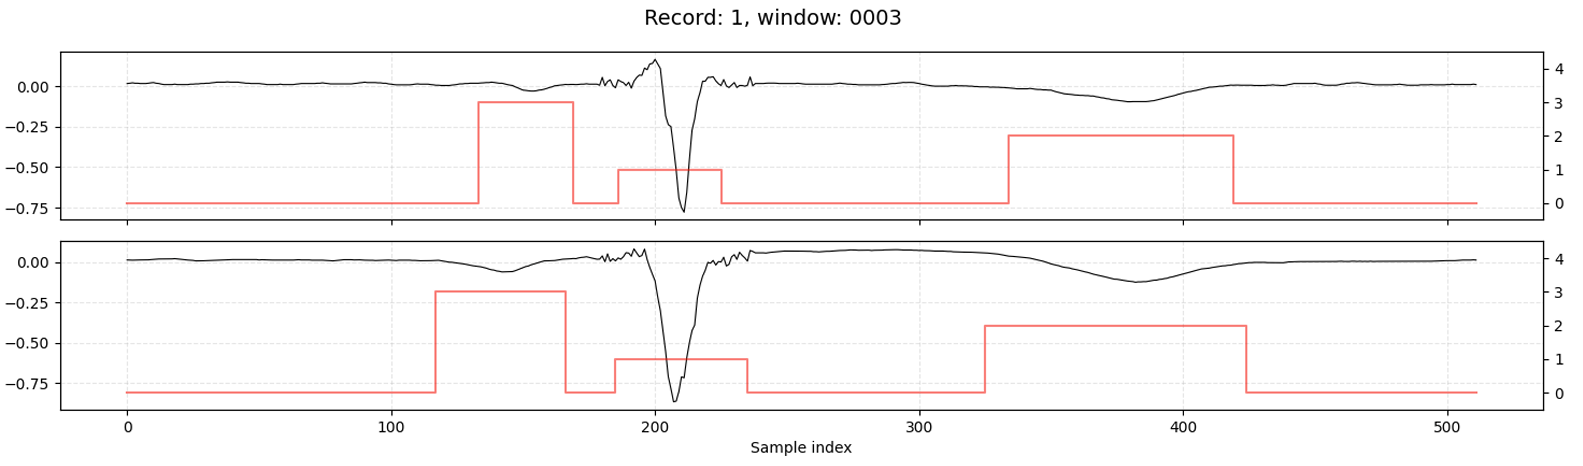
\includegraphics[width=1\textwidth]{segmentexample.png}
\caption{Пример участка сигнала ЭКГ с разметкой элементов кардиоцикла}
\label{fig:segmentexample}
\end{figure}

Наличие перекрытия уменьшает риск потери информативных фрагментов в случае,
когда границы сегментов или короткие события (например, часть комплекса QRS) попадают в область разрыва между соседними окнами: один и тот же временной участок будет присутствовать как минимум в двух соседних примерах. Это повышает стабильность обучения и снижает чувствительность модели к <<краевым>> эффектам при сегментации.


\subsubsection{Архитектура нейронной сети}

С помощью U-Net 1D архитектуры решается задача покомпонентной разметки (segmentation / sequence labeling) одномерного сигнала. Модель получает на вход тензор ЭКГ-сигнала
\[
x \in \mathbb{R}^{B \times C_{\text{in}} \times T},
\]
где $B$ --- размер пакета (batch size); $C_{\text{in}}$ --- число входных каналов (например ЭКГ отведений);
$T$ --- размер окна в отсчетах сигнала.

На выходе модель формирует логиты (logits) классов
\[
\text{logits} \in \mathbb{R}^{B \times C_{\text{cls}} \times T},
\]
где $C_{\text{cls}}$ --- число классов сегментации (\textit{фон / P / QRS / T}).
Впоследствии к логитам применяется $\mathrm{softmax}$ для получения вероятностей классов по каждому временному отсчету $t$.
Во всех реализациях используются одномерные свертки с ядром $k=3$ и дополнением (padding) равным единицей, а также одномерная пакетная нормализация и нелинейность выпрямителя (ReLU).

Согласно принципу формирования U-Net архитектур имеем, что энкодер уменьшает временное разрешение (downsampling) и увеличивает число каналов, а декодер восстанавливает временное разрешение (upsampling) и объединяет признаки с соответствующих уровней энкодера через skip-соединения.

\paragraph{Downsampling.}
Down-блоки используют оператор
\[
\texttt{MaxPool1d}(2),
\]
где значением аргумента является размерность окна субдискретизации (pooling). В результате длина последовательности уменьшается в 2 раза: $T \rightarrow T/2$. После операции субдискретизации выполняется сверточная обработка признаков.

\paragraph{Upsampling, sequence padding.}
Up-блоки используют транспонированную свертку
\[
\texttt{ConvTranspose1d}(k{=}2, s{=}2),
\]
где $k$ --- размер ядра, $s$ --- шаг (stride). Размер данных увеличивается в 2 раза: $T \rightarrow 2T$.
Из-за возможных несовпадений пространственной размерности между тензором, полученным в результате повышения дискретизации, и тензором пропускающего соединения в реализации архитектуры применяется операция симметричного дополнения (симметричного паддинга), для обеспечения корректной конкатенации
\[
x = \texttt{cat}\big[x_{\text{skip}},\, x_{\text{up}}\big]
\]
по оси отведений. Здесь $x_{\text{up}}$ --- признаки, полученные в результате повышения дискретизации в декодере, $x_{\text{skip}}$ --- признаки с соответствующего уровня энкодера
(до downsampling), а $\texttt{cat}[\cdot,\cdot]$ --- конкатенация по оси каналов ЭКГ сигнала.


\subsubsection{Структура блоков одномерной архитектуры U-Net}

\paragraph{DoubleConv1D.}
Базовый блок энкодера и декодера задается как:
\[
\text{DoubleConv}(x)=
\text{ReLU}\big(\text{BN}(\text{Conv}_{3}(x))\big)
\rightarrow
\text{ReLU}\big(\text{BN}(\text{Conv}_{3}(\cdot))\big),
\]
где $\text{Conv}_{3}(\cdot)$ --- одномерная свертка с ядром размера $3$; $\text{BN}(\cdot)$ --- пакетная нормализация; $\text{ReLU}(\cdot)$ --- функция активации. Стрелка обозначает композицию слоев на данном архитектурном уровне.

\paragraph{Down1D.}
Down-блок:
\[
\text{Down}(x) = \text{DoubleConv}(\text{MaxPool}(x)),
\]
где операция $MaxPool(\cdot)$ реализована как одномерное субдискретизирующее отображение, обеспечивающее двукратное сокращение временнóй протяженности сигнала.

\paragraph{Up1D.}
Up-блок:
\[
\text{Up}(x_{\text{low}}, x_{\text{skip}}) =
\text{DoubleConv}\left(\texttt{cat}\big[x_{\text{skip}},\, \text{UpConv}(x_{\text{low}})\big]\right),
\]
где $x_{\text{low}}$ --- признаки с более низким временным разрешением;
$x_{\text{skip}}$ --- признаки пропускающего соединения с соответствующего уровня энкодера;
$\text{UpConv}(\cdot)$ --- операция повышения дискретизации (upsampling);
$\texttt{cat}[\cdot,\cdot]$ --- конкатенация по каналам.

Пусть $F_0$ --- число базовых фильтров. Тогда число каналов по уровням U-Net:
$F_0,\,2F_0,\,4F_0,\,8F_0,\,16F_0$.

\paragraph{Encoder.}
\begin{align*}
x_1 &= \text{DoubleConv}(x) \in \mathbb{R}^{B \times F_0 \times T},\\
x_2 &= \text{Down}(x_1) \in \mathbb{R}^{B \times 2F_0 \times T/2},\\
x_3 &= \text{Down}(x_2) \in \mathbb{R}^{B \times 4F_0 \times T/4},\\
x_4 &= \text{Down}(x_3) \in \mathbb{R}^{B \times 8F_0 \times T/8},\\
x_5 &= \text{Down}(x_4) \in \mathbb{R}^{B \times 16F_0 \times T/16}.
\end{align*}
$x_i$ --- карты признаков на $i$-м уровне энкодера. Деление $T/2, T/4, \dots$ отражает редукцию временнóй протяженности сигнала в результате операции субдискретизации (pooling).
\paragraph{Bottleneck.}
\[
x_b = \text{DoubleConv}(x_5) \in \mathbb{R}^{B \times 16F_0 \times T/16},
\]
где $x_b$ --- признаки на нижнем уровне архитектуры U-Net (называемые bottleneck), содержащие наиболее контекстную информацию.

\paragraph{Decoder.}
\begin{align*}
x &= \text{Up}(x_b, x_4) \in \mathbb{R}^{B \times 8F_0 \times T/8},\\
x &= \text{Up}(x, x_3) \in \mathbb{R}^{B \times 4F_0 \times T/4},\\
x &= \text{Up}(x, x_2) \in \mathbb{R}^{B \times 2F_0 \times T/2},\\
x &= \text{Up}(x, x_1) \in \mathbb{R}^{B \times F_0 \times T}.
\end{align*}
В декодирующей части архитектуры на каждом уровне последовательно выполняются: повышение дискретизации (upsampling), конкатенация с признаками пропускающего соединения (skip-connection) и последующая сверточная обработка.

\paragraph{Выход сети.}
На финальном этап процедуры сегментации выполняется свертка $1\times1$:
\[
\text{logits} = \text{Conv}_{1}(x) \in \mathbb{R}^{B \times C_{\text{cls}} \times T},
\]
где $\text{Conv}_{1}(\cdot)$ --- одномерная свертка с размером ядра, равным единице, осуществляющая линейную классификацию для каждого временного отсчета $t$.

В представленной архитектуре реализуется иерархическое извлечение многомасштабных признаков посредством комбинации нисходящих и восходящих путей. На глубоких уровнях энкодера, благодаря последовательному уменьшению пространственного разрешения и расширению рецептивного поля, формируются признаки, обобщающие контекст на протяженных временных интервалах. В свою очередь, пропускающие соединения (skip connections), передающие активации с соответствующих уровней энкодера на соответствующие им уровни декодера, обеспечивают доступность пространственно-временной информации, что необходимо для локализации границ сегментов кардиоцикла.


\section{Параллельный алгоритм для решения задач глобальной оптимизации} \label{sec-PGSA}

Задача настройки гиперпараметров модели машинного обучения с математической точки зрения является задачей поиска глобального оптимума целевой метрики качества. 
В общем виде задача такого типа может быть записана следующим образом:
\begin{gather}
\varphi(y^\ast)=\min{\left\{\varphi(y):y\in D\right\}}, \label{eq_opt_problem}\\
D=\left\{y\in \mathbb{R}^N: a_i\leq y_i \leq b_i, \; a_i,b_i\in \mathbb{R}, \;  1\leq i \leq N\right\} \label{eq_D},
\end{gather}
где целевая функция $\varphi(y)$ является многоэкстремальной, задана в вида «черный ящик» (т.е. не имеет аналитического описания). Как и во многих других подходах к разработке методов глобальной оптимизации \cite{Evtushenko2013,Zilinskas2010,Pinter1996,Jones2009} будем предполагать, что $\varphi(y)$ в области поиска удовлетворяет условию Липшица с априори неизвестной константой $L, \; L<\infty,$, т.е. 
\[
\left|\varphi(y_1)-\varphi(y_2)\right|\leq L\left\|y_1-y_2\right\|,\; y_1,y_2 \in D.
\]

Для решения многомерных задач глобальной оптимизации в системе Globalizer используется редукция размерности на основе кривых Пеано \cite{Sergeyev2013, Strongin2000}. Кривая Пеано $y(x)$ непрерывно и однозначно отображает единичный отрезок $[0,1]$ на $N$-мерный гиперкуб $D$:
\[
D = \left\{ y \in \mathbb{R}^N: -2^{-1} \leq y_i \leq 2^{-1}, 1 \leq i \leq N \right\} = \left\{ y(x): 0 \leq x \leq 1 \right\}.
\]
С помощью такого отображения исходная многомерная задача (\ref{eq_opt_problem}) сводится к одномерной задаче
\[
\varphi(y^\ast)=\varphi(y(x^\ast))=\min{\left\{\varphi(y(x)): x\in[0,1]\right\}},
\]
где функция $\varphi(y(x))$ удовлетворяет равномерному условию Гёльдера
\[
\left|\varphi(y(x_1))-\varphi(y(x_2))\right|\leq H\left|x_1-x_2\right|^{1/N}
\]
с константой Гёльдера $H$, связанной с константой Липшица $L$ соотношением $H = 2L\sqrt{N+3}$.

Алгоритм глобального поиска (АГП) строит последовательность точек $x^i$, в которых проводятся поисковые испытания (здесь и далее будем называть процесс вычисления значения функции $f(x)=\varphi(y(x))$ \textit{испытанием}, а пару $\{x, z = f(x) = \varphi(y(x))\}$ --- результатом испытания). Пусть после выполнения $k$ испытаний накоплена поисковая информация $\Omega_k$, представленная в виде набора
\[
\Omega_k = \left\{ (x_i, y_i = y(x_i), z_i = \varphi(y_i)) : 1 \leq i \leq k \right\},
\]
где точки упорядочены по возрастанию $x$: $x_1 < x_2 < \ldots < x_k$.

Для выбора точки следующего испытания для каждого интервала $(x_{i-1}, x_i)$ вычисляется характеристика
\begin{equation}
R(i) = \Delta_i + \frac{(z_i - z_{i-1})^2}{(r\mu)^2\Delta_i} - 2\frac{z_{i-1} + z_i}{r\mu}, \label{eq_R}
\end{equation}
где $\Delta_i = (x_i - x_{i-1})^{1/N}$, $r>1$ --- параметр алгоритма, $\mu$ --- оценка константы Гёльдера, вычисляемая по формуле
\[
\mu = \max_{1 < i \leq k} \frac{|z_i - z_{i-1}|}{\Delta_i},
\]
причем если $\mu = 0$, то полагается $\mu = 1$.

Новое испытание проводится в точке $x^{k+1}$, принадлежащей интервалу с максимальной характеристикой $R(t) = \max\{R(i)\}$. Если правой точке этого интервала соответствует номер $t$ в множестве $\Omega_k$, то
\begin{equation}
x^{k+1} = \frac{x_t + x_{t-1}}{2} - \frac{\operatorname{sign}(z_t - z_{t-1})}{2r} \left( \frac{|z_t - z_{t-1}|}{\mu} \right)^N. \label{eq_x_new}
\end{equation}

Алгоритм завершает работу при выполнении условия $\Delta_t < \epsilon$, где $\epsilon > 0$ — заданная точность, либо при достижении максимального числа испытаний $K_{\max}$.


Для ускорения процесса оптимизации в системе Globalizer реализованы параллельные версии алгоритма. Основная идея распараллеливания заключается в одновременном проведении нескольких испытаний на разных вычислительных устройствах (процессах или потоках) \cite{Lebedev2022, Barkalov2016, globalizerSystem} . Вычислительная схема реализует принцип «мастер-рабочие», мастер-процесс выполняет основные шаги алгоритма глобального поиска: накапливает поисковую информацию, вычисляет оценку константы Гёльдера, определяет новые пробные точки и распределяет их между рабочими процессами. Рабочие процессы получают точки испытаний от главного процесса, вычисляют значения целевой функции в этих точках и отправляют результаты мастеру.

В синхронной схемы вычислений переход к следующей итерации осуществляется только после завершения всех $p$ испытаний текущей итерации. Достоинством синхронной схемы является простота реализации, однако при значительном разбросе времени вычисления целевой функции в разных точках возможны простои вычислительных ресурсов.

Для устранения недостатков синхронной схемы разработана асинхронная версия параллельного алгоритма. Ее ключевая идея заключается в том, чтобы не ожидать завершения всех испытаний текущей итерации, а отправлять новую точку на вычисление сразу после получения результата от любого рабочего процесса.

Пусть в нашем распоряжении имеется $p+1$ вычислительных процессов: один мастер (процесс 0) и $p$ рабочих процессов. В начале поиска мастер инициирует параллельное выполнение $p$ испытаний в различных точках области поиска (начальные точки распределяются равномерно или случайным образом).

Предположим, что выполнено $k \geq 0$ испытаний и рабочие процессы выполняют испытания в точках $x^{k+1}, x^{k+2}, \ldots, x^{k+p}$. Обозначим $I_k = \{x^{k+1}, x^{k+2}, \ldots, x^{k+p}\}$ --- множество прообразов точек, в которых испытания начаты, но еще не завершены.

Алгоритм выполнения асинхронной схемы включает следующие шаги.

\textbf{Шаг 1.} Перенумеровать множество $X_k = \{x^1, x^2, \ldots, x^{k+p}\}$, содержащее все прообразы точек, в которых испытания либо завершены, либо выполняются, в порядке возрастания:
\[
0 = x_1 < x_2 < \ldots < x_{k+p} = 1.
\]

\textbf{Шаг 2.} Вычислить оценки:
\[
M_1 = \max\left\{ \frac{|z_i - z_{i-1}|}{(x_i - x_{i-1})^{1/N}} : x_{i-1} \notin I_k, x_i \notin I_k, 2 \leq i \leq k+p \right\},
\]
\[
M_2 = \max\left\{ \frac{|z_{i+1} - z_{i-1}|}{(x_{i+1} - x_{i-1})^{1/N}} : x_i \in I_k, 2 \leq i < k+p \right\},
\]
\[
M = \max\{M_1, M_2\},
\]
где $z_i = \varphi(y(x_i))$, если $x_i \notin I_k$. Если $M = 0$, положить $M = 1$.

\textbf{Шаг 3.} Для каждого интервала $(x_{i-1}, x_i)$ с $x_{i-1} \notin I_k$, $x_i \notin I_k$ вычислить характеристику
\[
R(i) = \Delta_i + \frac{(z_i - z_{i-1})^2}{(rM)^2\Delta_i} - 2\frac{z_i + z_{i-1}}{rM},
\]
где $\Delta_i = (x_i - x_{i-1})^{1/N}$.

\textbf{Шаг 4.} Выбрать интервал $(x_{t-1}, x_t)$ с максимальной характеристикой:
\[
R(t) = \max\{ R(i) : x_{i-1} \notin I_k, x_i \notin I_k, 2 \leq i \leq k+p \}.
\]

\textbf{Шаг 5.} Определить новую точку для проведения испытания:
\[
x^{k+p+1} = \frac{x_t + x_{t-1}}{2} - \operatorname{sign}(z_t - z_{t-1}) \frac{1}{2r} \left( \frac{|z_t - z_{t-1}|}{M} \right)^N.
\]

Мастер добавляет точку $x^{k+p+1}$ к множеству $I_k$ и отправляет ее освободившемуся рабочему процессу для проведения нового испытания.

Алгоритм завершает работу при выполнении условия $\Delta_t < \varepsilon$ или $k+p > K_{\max}$.

Основное преимущество асинхронной схемы заключается в минимизации простоев вычислительных ресурсов: мастер обрабатывает результаты по мере их поступления, а рабочие процессы немедленно получают новые задания после завершения предыдущих.


\section{Результаты численных экспериментов}
\label{sec-result}

Вычислительные эксперименты проводились на узле суперкомпьютера <<Лобачевский>> в следующей конфигурации: операционная система Linux CentOS 8.2, 2 процессора Intel Xeon Platinum 8558 2.1/4GHz (48 ядер каждый), оперативная память 2048 Gb, 8 графических ускорителей Nvidia RTX PRO 6000. 
Рассмотренные алгоритмы оптимизации реализованы на С++, использовался компилятор Intel С++ Сompiler 2023 с поддержкой OpenMP. Обучение моделей искусственного интеллекта проводились с использованием фреймворка PyTorch, использовался Python 3.12.


Для проведения экспериментов использовались две нейросетевые модели, описанные в разделе 2: модель классификации на основе MobileNetV3 Small и модель сегментации на основе одномерной U-Net. Вычислительные затраты на одну итерацию оптимизации (одно испытание) составляли:
\begin{itemize}
    \item для задачи классификации --- обучение модели в течение 100 эпох с оценкой качества на валидационной выборке;
    \item для задачи сегментации --- обучение модели в течение 40 эпох с вычислением метрики качества.
\end{itemize}

Параметры запуска алгоритма глобального поиска в системе Globalizer:
\begin{itemize}
    \item параметр надежности $r = 10$;
    \item точность глобального поиска $\varepsilon = 10^{-2}$;
    \item максимальное число поисковых испытаний $K_{\max} = 320$;
    \item плотность построения развертки $m = 10$.
\end{itemize}

Для синхронной и асинхронной схем распараллеливания использовалось схема мастер-рабочий (один мастер и несколько рабочих), всего использовалось MPI процессов: 1, 3, 5, 9, 17, 33. Целевой метрикой  выбрана F1-мера.


На первом этапе экспериментов выполнялась оптимизация гиперпараметров модели классификации ЭКГ-сигналов. Варьируемыми параметрами являлись:
\begin{itemize}
    \item число классифицирующих нейронов в выходном слое: $f \in [80, 200]$;
    \item Вероятность отключения нейронов: $p \in [0.0, 1.0]$.
\end{itemize}

Для визуализации характера целевой функции был построен график (рис.~\ref{fig_classification_surface}), на котором представлена интерполяция значений целевой метрики в зависимости от числа нейронов и вероятность отключения нейронов. Видно, что функция имеет выраженный многоэкстремальный характер, что подтверждает необходимость применения методов глобальной оптимизации.

\begin{figure}[ht]
\centering
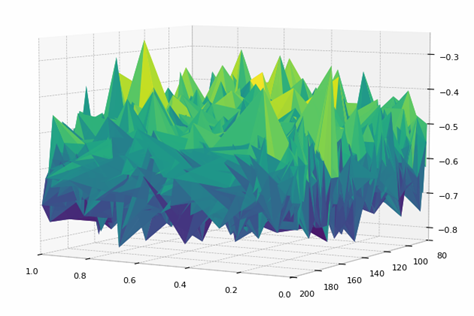
\includegraphics[width=0.8\textwidth]{classification_surface.png}
\caption{Поверхность целевой функции для задачи классификации ЭКГ в зависимости от числа нейронов и вероятности Dropout}
\label{fig_classification_surface}
\end{figure}


В табл.~\ref{tab_classification_scalability} представлены результаты масштабирования параллельных алгоритмов при оптимизации гиперпараметров модели классификации. Для каждого количества процессов указано найденное значение целевой метрики и достигнутое ускорение относительно последовательного запуска, длительность которого составила 11.3 минуты.

\begin{table}[ht]
\caption{Результаты масштабирования для задачи классификации ЭКГ}
\label{tab_classification_scalability}
\centering
\begin{tabular}{|c|c|c|c|c|}
\hline
Число процессов & \multicolumn{2}{c|}{Синхронная схема} & \multicolumn{2}{c|}{Асинхронная схема} \\
\cline{2-5}
& $F_1^{\mathrm{macro}}$ & Ускорение & $F_1^{\mathrm{macro}}$ & Ускорение \\
\hline
1  & 0.78 & 1.00   &  0.78 &  1.00   \\
3  & 0.75 & 1.98   &  0.78 &  1.94   \\
5  & 0.80 & 3.91   &  0.78 &  3.65   \\
9  & 0.78 & 7.32   &  0.78 &  10.11  \\
17 & 0.78 & 12.81  &  0.78 &  22.91  \\
33 & 0.78 & 18.07  &  0.83 &  15.94  \\

\hline
\end{tabular}

\end{table}

Анализ полученных результатов показывает, что асинхронная схема распараллеливания демонстрирует более высокую эффективность по сравнению с синхронной схемой, особенно при увеличении числа процессов. Это объясняется тем, что время обучения нейросетевой модели может варьироваться в зависимости от конкретных значений гиперпараметров, и асинхронная схема позволяет минимизировать простои вычислительных ресурсов. При этом при разном количестве процессов мы получаем разные траектории, в которых суммарное время вычислений  значительно отличается.

На втором этапе экспериментов выполнялась оптимизация гиперпараметров модели сегментации ЭКГ-сигналов на основе одномерной U-Net. Варьируемыми параметрами являлись:
\begin{itemize}
    \item Вероятность отключения нейронов: $p \in [0.0, 1.0]$.;
    \item количество уровней энкодера/декодера: $depth \in [3, 5]$.
\end{itemize}


Основной метрикой качества являлась macro-$F_1$ без фонового класса.
Для каждого класса $c$ вычислялись precision и recall:
\[
\mathrm{Precision}_c=\frac{TP_c}{TP_c+FP_c}, \qquad
\mathrm{Recall}_c=\frac{TP_c}{TP_c+FN_c},
\]
а затем $F_1$-мера:
\[
F_{1,c} = \frac{2\cdot \mathrm{Precision}_c\cdot \mathrm{Recall}_c}{\mathrm{Precision}_c+\mathrm{Recall}_c}.
\]
Здесь $TP_c, FP_c, FN_c$ --- число истинно-положительных, ложноположительных и ложноотрицательных предсказаний класса $c$,
подсчитанных по всем отсчетам времени $t$ на всей выборке.

В рамках эксперимента $F_1$-мера рассчитывался по точному совпадению меток на каждом отсчете (без временного допуска).
Итоговая метрика для сравнения моделей вычислялась как среднее по классам без фона:
\[
F_1^{\mathrm{macro}} = \frac{1}{C_{\mathrm{cls}}-1}\sum_{c=1}^{C_{\mathrm{cls}}-1} F_{1,c}.
\]


%На рис.~\ref{fig_segmentation_surface} представлен график поверхности целевой 
%функции для задачи сегментации. Характер поверхности также является 
%многоэкстремальным, что подтверждает сложность задачи выбора оптимальных 
%гиперпараметров.
%\begin{figure}[ht]
%\centering
%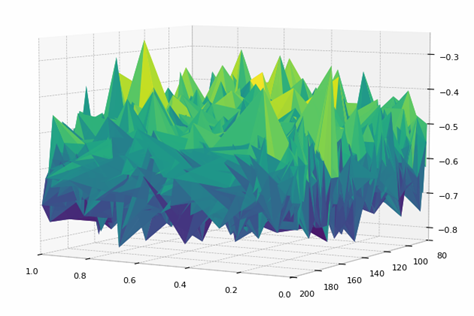
\includegraphics[width=0.8\textwidth]{classification_surface.png}
%\caption{Поверхность целевой функции для задачи сегментации ЭКГ (средняя F1-
%мера) в зависимости от числа базовых фильтров и глубины сети}
%\label{fig_segmentation_surface}
%\end{figure}

В табл.~\ref{tab_segmentation_scalability} представлены результаты масштабирования параллельных алгоритмов при оптимизации гиперпараметров модели сегментации. При установленном ограничении на число испытаний $K_{max} = 320$ длительность последовательного запуска составила 5.5 часов.

\begin{table}[ht]
\caption{Результаты масштабирования для задачи сегментации ЭКГ}
\label{tab_segmentation_scalability}
\centering
\begin{tabular}{|c|c|c|c|c|}
\hline
Число процессов & \multicolumn{2}{c|}{Синхронная схема} & \multicolumn{2}{c|}{Асинхронная схема} \\
\cline{2-5}
& $F_1^{\mathrm{macro}}$ & Ускорение & $F_1^{\mathrm{macro}}$ & Ускорение \\
\hline
1  & 0.80  & 1.00   & 0.80  & 1.00  \\
3  & 0.79   & 1.87    & 0.79  & 1.85  \\
5  & 0.80   & 3.10    & 0.79  & 3.38  \\
9  & 0.80  & 5.69   & 0.80  & 6.34  \\
17 & 0.79  & 9.46   & 0.79  & 15.68 \\
33 & 0.80  & 13.88  & 0.79  & 14.29 \\
\hline
\end{tabular}

\end{table}

Сравнение результатов для задач классификации и сегментации показывает, что эффективность асинхронной схемы вычислений выше для задачи сегментации, что связано с большей вычислительной трудоемкостью одного испытания (обучение модели сегментации требует больше времени вследствие большей глубины сети и большего объема обрабатываемых данных).


\section{Заключение}
\label{sec-conclusion}

В работе рассмотрена задача оптимизации гиперпараметров нейросетевых моделей классификации и сегментации сигналов ЭКГ с использованием параллельного алгоритма глобального поиска, реализованного в программной системе Globalizer. Для задачи классификации (модель MobileNetV3 Small) варьировались число нейронов (80--200) и вероятность отключения нейронов (0.0--1.0), достигнуто значение целевой метрики macro-$F_1$, равное 0.83. Для задачи сегментации (одномерная U-Net) варьировались глубина сети (3--5) и Dropout (0.0--1.0), достигнуто значение целевой метрики macro-$F_1$ равное 0.80. Исследована эффективность синхронной и асинхронной схем распараллеливания на суперкомпьютере <<Лобачевский>>. Асинхронная схема показала более высокую эффективность: при 17 процессах ускорение составило 22.91 для классификации и 15.68 для сегментации. Полученные результаты подтверждают, что асинхронный алгоритм глобальной оптимизации, реализованный в системе Globalizer, является эффективным инструментом настройки гиперпараметров нейронных сетей для задач медицинской диагностики.

\begin{biblio}


\bibitem{Ansari2023}
Ansari~Y., Mourad~O., Qaraqe~K., Serpedin~E. Deep learning for ECG arrhythmia detection and classification: an overview of progress for period 2017–2023 // Frontiers in Physiology. 2023. Vol.~14. 1246746.

\bibitem{Seenivasan2025}
Seenivasan~D., Sakthivel~K. Patch-Based ECG Segmentation for Arrhythmia Classification Using Hybrid Deep Learning // Information Technology and Control. 2025. Vol.~54, No.~4. P.~1189--1205.

\bibitem{Xiao2023}
Xiao~Q., Lee~K., Mokhtar~S.A., Ismail~I., Pauzi~A.L.B.M., Zhang~Q., Lim~P.Y. Deep learning-based ECG arrhythmia classification: A systematic review // Applied Sciences. 2023. Vol.~13, No.~8. 4964.

\bibitem{Huang2023}
Huang~Y., Li~H., Yu~X. A novel time representation input based on deep learning for ECG classification // Biomedical Signal Processing and Control. 2023. Vol.~83. 104628.

\bibitem{optuna}
Akiba~T., Sano~S., Yanase~T.,  Ohta~T., Koyama~M. Optuna: A Next-Generation Hyperparameter Optimization Framework // Proceedings of the 25th ACM SIGKDD International Conference on Knowledge Discovery \& Data Mining. 2019. P.~2623–-2631. DOI:~\href{https://dl.acm.org/doi/10.1145/3292500.3330701}{10.1145/3292500.3330701}

\bibitem{hyperopt}
Bergstra~J., Yamins~D., Cox~D.D. Making a Science of Model Search: Hyperparameter Optimization in Hundreds of Dimensions for Vision Architectures // Proceedings of the 30th International Conference on Machine Learning. 2013. P.~115--123.

\bibitem{Yang2013}
Yang~X.-S. Engineering optimization: An introduction with metaheuristic applications. Hoboken: John Wiley \& Sons, 2013. 384~p.

\bibitem{Gendreau2010}
Gendreau~M., Potvin~J.-Y. (Eds.) Handbook of metaheuristics. 2nd ed. New York: Springer, 2010. 640~p.

\bibitem{Eiben2015}
Eiben~A.E., Smith~J.E. Introduction to evolutionary computing. 2nd ed. Berlin: Springer, 2015. 294~p.

\bibitem{Kvasov2018}
Квасов~Д.Е., Сергеев~Я.Д. Методы липшицевой глобальной оптимизации в задачах управления // АиТ. 2013. № 9. C. 3--19. DOI:~\href{https://doi.org/10.1134/S0005117913090014}{10.1134/S0005117913090014}
%Kvasov~D.E., Mukhametzhanov~M.S. Metaheuristic vs. deterministic global optimization algorithms: The univariate case // Applied Mathematics and Computation. 2018. Vol.~318. P.~245--259. DOI:~\href{http://dx.doi.org/10.1016/j.amc.2017.05.014}{10.1016/j.amc.2017.05.014}.

\bibitem{Sergeyev2006}
Сергеев~Я.Д., Квасов~Д.Е. Диагональные методы глобальной оптимизации. М.: ФИЗМАТЛИТ, 2008. 352 с.
%Sergeyev~Y.D., Kvasov~D.E. Global search based on efficient diagonal partitions and a set of Lipschitz constants // SIAM Journal on Optimization. 2006. Vol.~16, No.~3. P.~910--937. DOI:~\href{http://dx.doi.org/10.1137/040621132}{10.1137/040621132}.


\bibitem{Zilinskas2008}
Žilinskas~A. Branch and bound algorithm for multidimensional scaling with city-block metric // Journal of Global Optimization. 2008. Vol.~43, No.~2--3. P.~357--372. DOI:~\href{http://dx.doi.org/10.1007/s10898-008-9306-x}{10.1007/s10898-008-9306-x}.

\bibitem{Strongin2000}
Strongin~R.G., Sergeyev~Y.D. Global optimization with non-convex constraints. Sequential and parallel algorithms. Dordrecht: Kluwer Academic Publishers, 2000. 416~p. DOI:~\href{https://doi.org/10.1007/978-1-4615-4677-1}{10.1007/978-1-4615-4677-1}.

\bibitem{Strongin2018}
Strongin~R., Gergel~V., Barkalov~K., Sysoyev~A. Generalized parallel computational schemes for time-consuming global optimization //  Lobachevskii Journal of Mathematics. 2018. Vol.~39, No.~4 P.~576--586. DOI:~\href{http://dx.doi.org/10.1134/S1995080218040133}{10.1134/S1995080218040133}.

\bibitem{Kalyakulina2020}
Kalyakulina~A.I., Yusipov~I.I., Moskalenko~V.A., Nikolskiy~A.V., Kozlov~K.A., Zudov~K.A., Ivanchenko~M.V. LUDB: a new open-access validation tool for electrocardiogram delineation algorithms // IEEE Access. 2020. Vol.~8. P.~186181--186190. DOI:~\href{https://doi.org/10.1109/ACCESS.2020.3029376}{10.1109/ACCESS.2020.3029376}.

%\bibitem{Piyavskii1972} 
%Пиявский~С.А. Один алгоритм отыскания абсолютного экстремума функции // Ж. вычисл. матем. и матем. физ. 1972. T.~12, №~4. С.~888--896.

%\bibitem{Shubert1972}
%Shubert~B. A sequential method seeking the global maximum of a function // SIAM Journal on Numerical Analysis. 1972. Vol.~9, No.~3. P.~379--388.

\bibitem{Evtushenko2013}
Евтушенко~Ю.Г., Малкова~В.У., Станевичюс~А.-И.А. Параллельный поиск глобального экстремума функций многих переменных // Ж. вычисл. матем. и матем. физ. 2009. Т.~49, №~2. C.~255--269. DOI:~\href{https://doi.org/10.1134/S0005117907050062}{10.1134/S0005117907050062}.
%Evtushenko~Yu.G., Posypkin~M.A. A deterministic approach to global box-constrained optimization // Optimization Letters. 2013. Vol.~7, No.~4. P.~819--829. DOI:~\href{http://dx.doi.org/10.1007/s11590-012-0452-1}{10.1007/s11590-012-0452-1}.

\bibitem{Zilinskas2010}
Žilinskas~A., Žilinskas~J. Global optimization based on a statistical model and simplicial partitioning // Computers \& Operations Research. 2010. Vol.~37, No.~10. P.~1759--1767. DOI:~\href{http://dx.doi.org/10.1016/S0898-1221(02)00206-7}{10.1016/S0898-1221(02)00206-7}.

\bibitem{Pinter1996}
Pintér~J.D. Global optimization in action: Continuous and Lipschitz optimization: Algorithms, implementations and applications. Dordrecht: Kluwer Academic Publishers, 1996. 480~p.

\bibitem{Jones2009}
Jones~D.R. The DIRECT global optimization algorithm // Encyclopedia of Optimization. Boston: Springer, 2009. P.~725--735. DOI:~\href{https://doi.org/10.1007/978-0-387-74759-0_128}{10.1007/978-0-387-74759-0\_128}

\bibitem{Sergeyev2013}
Стронгин~Р.Г., Гергель~В.П., Гришагин~В.А., Баркалов~К.А. Параллельные вычисления в задачах глобальной оптимизации. М.: Изд-во МГУ, 2013.
%Sergeyev~Y.D., Strongin~R.G., Lera~D. Introduction to global optimization exploiting space-filling curves. New York: Springer, 2013. 148~p. DOI:~\href{http://dx.doi.org/10.1007/978-1-4614-8042-6}{10.1007/978-1-4614-8042-6}.

\bibitem{Lebedev2022}
Barkalov~K., Lebedev~I., Karchkov~D. Analysis and elimination of bottlenecks in parallel algorithm for solving global optimization problems // Lecture Notes in Computer Science. 2022. Vol.~13708. P.~18--32. DOI:~\href{https://doi.org/10.1007/978-3-031-22941-1_2}{10.1007/978-3-031-22941-1\_2}.


\bibitem{Barkalov2016} 
Barkalov~K., Lebedev~I. Solving multidimensional global optimization problems using graphics accelerators // Communications in Computer and Information Science. 2016. Vol.~687. P.~224--235. DOI:~\href{http://dx.doi.org/10.1007/978-3-319-55669-7_18}{10.1007/978-3-319-55669-7\_18}.


\bibitem{globalizerSystem}
Gergel~V., Barkalov~K., Sysoyev~A. A novel supercomputer software system for solving time-consuming global optimization problems // Numerical Algebra, Control \& Optimization. 2018. Vol.~8, No.~1. P.~47--62. DOI:~\href{http://dx.doi.org/10.3934/naco.2018003}{10.3934/naco.2018003}.





%\bibitem{Sergeyev2018} Sergeyev~Y.D., Kvasov~D.E., Mukhametzhanov~M.S. On the efficiency of nature-inspired metaheuristics in expensive global optimization with limited budget // Scientific Reports. 2018. Vol.~8, Article number:~453. DOI:~\href{http://dx.doi.org/10.1038/s41598-017-18940-4}{10.1038/s41598-017-18940-4}.


%\bibitem{Himmelblau75} Химмельблау~Д. Прикладное нелинейное программирование. М.: Мир, 1975. 535~с.


%\bibitem{eremin} Ерёмин~И.И. Фейеровские методы для задач выпуклой и линейной оптимизации. Челябинск: Изд-во ЮУрГУ, 2009. 200~с.

%\bibitem{levin} Левин~В.К. Отечественные суперкомпьютеры семейства МВС. URL:~\href{http://parallel.ru/mvs/levin.htm}{http://parallel.ru/mvs/levin.htm} (дата обращения: 27.05.2012).

%\bibitem{sokolinsky} Соколинский~Л.Б. Организация параллельного выполнения запросов в многопроцессорной машине баз данных с иерархической архитектурой // Программирование. 2001. №~6. С.~13--29.


%\bibitem{roosta} Roosta~S.H. Parallel Processing and Parallel Algorithms: Theory and Computation. Springer, 2000. 566~p. DOI:~\href{http://dx.doi.org/10.1007/978-1-4612-1220-1}{10.1007/978-1-4612-1220-1}.

%\bibitem{cadez} Cadez~I., Heckerman~D., Meek~C., et al. Visualization of Navigation Patterns on a Web Site Using Model Based Clustering. Technical Report MSR TR 00 18. Microsoft Research. 2000. URL:~\href{http://research.microsoft.com/pubs/69752/tr-2000-18.pdf}{http://research.microsoft.com/pubs/69752/tr-2000-18.pdf} (accessed:~13.12.2009). 

%\bibitem{levshin} Levshin~D.V., Markov~A.S. Algorithms for Integrating PostgreSQL with the Semantic Web // Programming and Computer Software. 2009. Vol.~35, No.~3. P.~136--144. DOI:~\href{http://dx.doi.org/10.1134/s0361768809030025}{10.1134/s0361768809030025}.

%\bibitem{stonebraker} Stonebraker~M., Kemnitz~G. The POSTGRES Next-generation Database Management System // Communications of the ACM. 1991. Vol.~34, No.~10. P.~78--92. DOI:~\href{http://dx.doi.org/10.1145/125223.125262}{10.1145/125223.125262}.

\end{biblio}

\end{document}